\documentclass{standalone}
\usepackage{tikz}
\usetikzlibrary{patterns, positioning}


\begin{document}
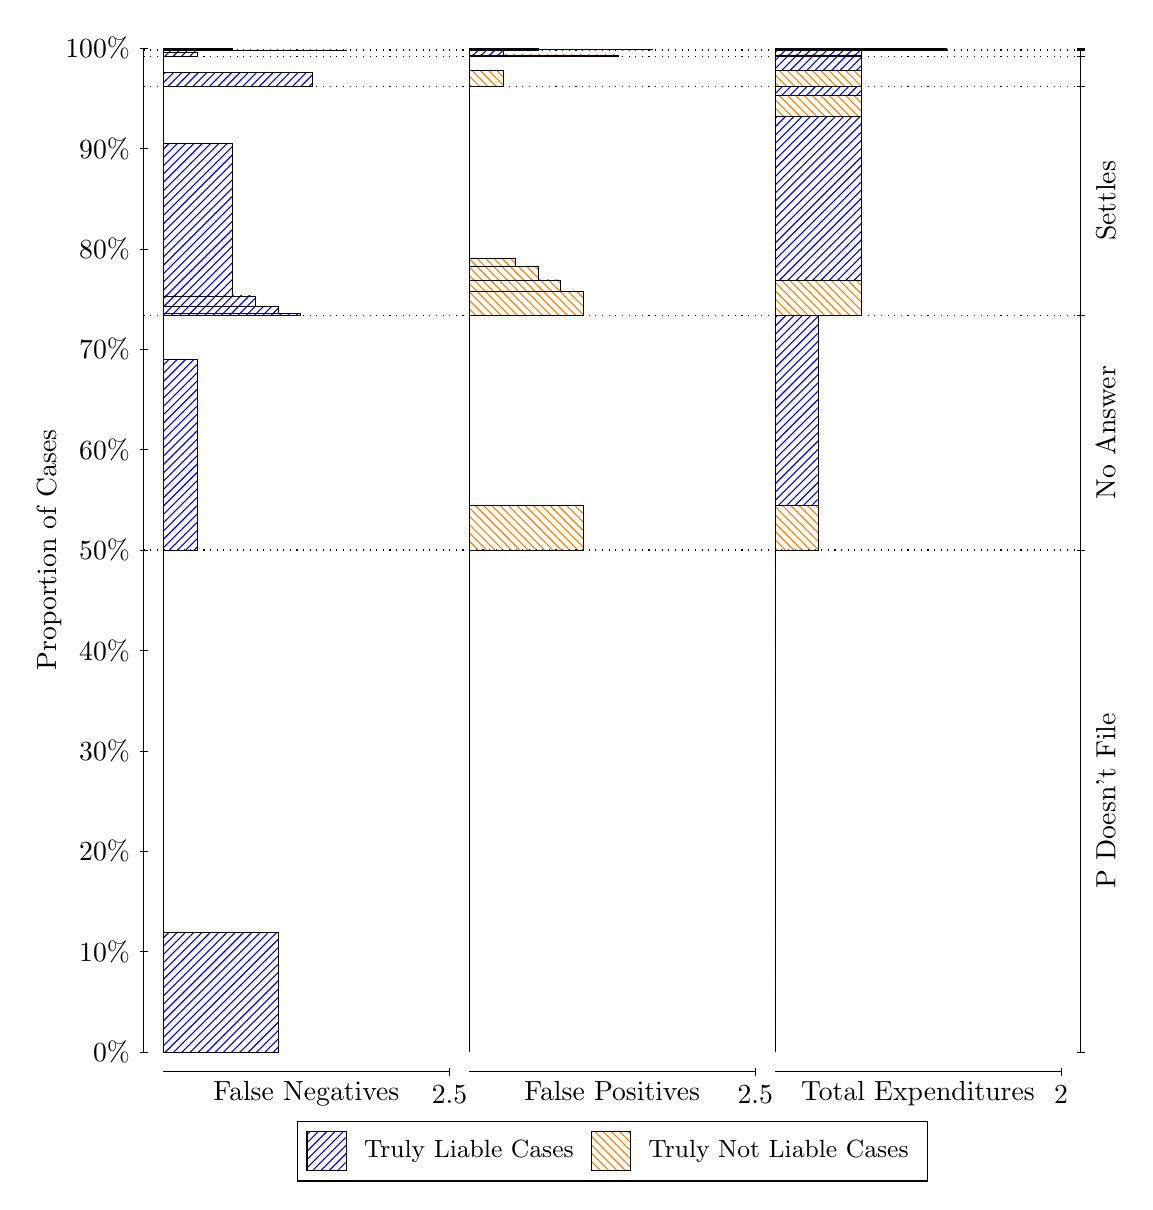
\begin{tikzpicture}
\draw[black, very thin] (1.5,1.75) -- (1.5,14.5);
\node[rotate=90, text=black, anchor=center] at (0.3, 8.125) {Proportion of Cases};
\draw[black, very thin] (1.45,1.75) -- (1.55,1.75);
\node[text=black, anchor=east] at (1.45, 1.75) {0\%};
\draw[black, very thin] (1.45,3.025) -- (1.55,3.025);
\node[text=black, anchor=east] at (1.45, 3.025) {10\%};
\draw[black, very thin] (1.45,4.3) -- (1.55,4.3);
\node[text=black, anchor=east] at (1.45, 4.3) {20\%};
\draw[black, very thin] (1.45,5.575) -- (1.55,5.575);
\node[text=black, anchor=east] at (1.45, 5.575) {30\%};
\draw[black, very thin] (1.45,6.85) -- (1.55,6.85);
\node[text=black, anchor=east] at (1.45, 6.85) {40\%};
\draw[black, very thin] (1.45,8.125) -- (1.55,8.125);
\node[text=black, anchor=east] at (1.45, 8.125) {50\%};
\draw[black, very thin] (1.45,9.4) -- (1.55,9.4);
\node[text=black, anchor=east] at (1.45, 9.4) {60\%};
\draw[black, very thin] (1.45,10.675) -- (1.55,10.675);
\node[text=black, anchor=east] at (1.45, 10.675) {70\%};
\draw[black, very thin] (1.45,11.95) -- (1.55,11.95);
\node[text=black, anchor=east] at (1.45, 11.95) {80\%};
\draw[black, very thin] (1.45,13.225) -- (1.55,13.225);
\node[text=black, anchor=east] at (1.45, 13.225) {90\%};
\draw[black, very thin] (1.45,14.5) -- (1.55,14.5);
\node[text=black, anchor=east] at (1.45, 14.5) {100\%};

\draw[black, very thin] (13.4,1.75) -- (13.4,14.5);
\draw[black, very thin] (13.35,1.75) -- (13.45,1.75);
\node[anchor=west] at (13.35, 1.75) {};
\draw[black, very thin] (13.35,8.1251) -- (13.45,8.1251);
\node[anchor=west] at (13.35, 8.1251) {};
\draw[black, very thin] (13.35,11.105) -- (13.45,11.105);
\node[anchor=west] at (13.35, 11.105) {};
\draw[black, very thin] (13.35,14.013) -- (13.45,14.013);
\node[anchor=west] at (13.35, 14.013) {};
\draw[black, very thin] (13.35,14.392) -- (13.45,14.392);
\node[anchor=west] at (13.35, 14.392) {};
\draw[black, very thin] (13.35,14.47) -- (13.45,14.47);
\node[anchor=west] at (13.35, 14.47) {};
\draw[black, very thin] (13.35,14.48) -- (13.45,14.48);
\node[anchor=west] at (13.35, 14.48) {};
\draw[black, very thin] (13.35,14.5) -- (13.45,14.5);
\node[anchor=west] at (13.35, 14.5) {};

\draw[black, very thin, pattern color=blue, pattern=north east lines] (1.75,1.75) rectangle (3.2033,3.2718);
\draw[black, very thin, pattern color=orange, pattern=north west lines] (1.75,3.2718) rectangle (1.75,8.1251);
\draw[black, very thin, pattern color=blue, pattern=north east lines] (1.75,8.1251) rectangle (2.186,10.542);
\draw[black, very thin, pattern color=orange, pattern=north west lines] (1.75,10.542) rectangle (1.75,11.105);
\draw[black, very thin, pattern color=blue, pattern=north east lines] (1.75,11.105) rectangle (3.494,11.127);
\draw[black, very thin, pattern color=blue, pattern=north east lines] (1.75,11.127) rectangle (3.2033,11.215);
\draw[black, very thin, pattern color=blue, pattern=north east lines] (1.75,11.215) rectangle (2.9127,11.353);
\draw[black, very thin, pattern color=blue, pattern=north east lines] (1.75,11.353) rectangle (2.622,13.288);
\draw[black, very thin, pattern color=orange, pattern=north west lines] (1.75,13.288) rectangle (1.75,14.013);
\draw[black, very thin, pattern color=blue, pattern=north east lines] (1.75,14.013) rectangle (3.6393,14.189);
\draw[black, very thin, pattern color=orange, pattern=north west lines] (1.75,14.189) rectangle (1.75,14.392);
\draw[black, very thin, pattern color=blue, pattern=north east lines] (1.75,14.392) rectangle (2.186,14.45);
\draw[black, very thin, pattern color=orange, pattern=north west lines] (1.75,14.45) rectangle (1.75,14.47);
\draw[black, very thin, pattern color=blue, pattern=north east lines] (1.75,14.47) rectangle (4.0753,14.474);
\draw[black, very thin, pattern color=orange, pattern=north west lines] (1.75,14.474) rectangle (1.75,14.48);
\draw[black, very thin, pattern color=blue, pattern=north east lines] (1.75,14.48) rectangle (2.622,14.495);
\draw[black, very thin, pattern color=orange, pattern=north west lines] (1.75,14.495) rectangle (1.75,14.5);
\draw[black, very thin, pattern color=orange, pattern=north west lines] (5.6333,1.75) rectangle (5.6333,6.6033);
\draw[black, very thin, pattern color=blue, pattern=north east lines] (5.6333,6.6033) rectangle (5.6333,8.1251);
\draw[black, very thin, pattern color=orange, pattern=north west lines] (5.6333,8.1251) rectangle (7.0867,8.6876);
\draw[black, very thin, pattern color=blue, pattern=north east lines] (5.6333,8.6876) rectangle (5.6333,11.105);
\draw[black, very thin, pattern color=orange, pattern=north west lines] (5.6333,11.105) rectangle (7.0867,11.405);
\draw[black, very thin, pattern color=orange, pattern=north west lines] (5.6333,11.405) rectangle (6.796,11.555);
\draw[black, very thin, pattern color=orange, pattern=north west lines] (5.6333,11.555) rectangle (6.5053,11.723);
\draw[black, very thin, pattern color=orange, pattern=north west lines] (5.6333,11.723) rectangle (6.2147,11.83);
\draw[black, very thin, pattern color=blue, pattern=north east lines] (5.6333,11.83) rectangle (5.6333,14.013);
\draw[black, very thin, pattern color=orange, pattern=north west lines] (5.6333,14.013) rectangle (6.0693,14.217);
\draw[black, very thin, pattern color=blue, pattern=north east lines] (5.6333,14.217) rectangle (5.6333,14.392);
\draw[black, very thin, pattern color=orange, pattern=north west lines] (5.6333,14.392) rectangle (7.5227,14.412);
\draw[black, very thin, pattern color=blue, pattern=north east lines] (5.6333,14.412) rectangle (6.0693,14.47);
\draw[black, very thin, pattern color=orange, pattern=north west lines] (5.6333,14.47) rectangle (6.5053,14.475);
\draw[black, very thin, pattern color=blue, pattern=north east lines] (5.6333,14.475) rectangle (5.6333,14.48);
\draw[black, very thin, pattern color=orange, pattern=north west lines] (5.6333,14.48) rectangle (7.9587,14.485);
\draw[black, very thin, pattern color=blue, pattern=north east lines] (5.6333,14.485) rectangle (6.5053,14.5);
\draw[black, very thin, pattern color=orange, pattern=north west lines] (9.5167,1.75) rectangle (9.5167,6.6033);
\draw[black, very thin, pattern color=blue, pattern=north east lines] (9.5167,6.6033) rectangle (9.5167,8.1251);
\draw[black, very thin, pattern color=orange, pattern=north west lines] (9.5167,8.1251) rectangle (10.062,8.6876);
\draw[black, very thin, pattern color=blue, pattern=north east lines] (9.5167,8.6876) rectangle (10.062,11.105);
\draw[black, very thin, pattern color=orange, pattern=north west lines] (9.5167,11.105) rectangle (10.607,11.555);
\draw[black, very thin, pattern color=blue, pattern=north east lines] (9.5167,11.555) rectangle (10.607,13.628);
\draw[black, very thin, pattern color=orange, pattern=north west lines] (9.5167,13.628) rectangle (10.607,13.903);
\draw[black, very thin, pattern color=blue, pattern=north east lines] (9.5167,13.903) rectangle (10.607,14.013);
\draw[black, very thin, pattern color=orange, pattern=north west lines] (9.5167,14.013) rectangle (10.607,14.217);
\draw[black, very thin, pattern color=blue, pattern=north east lines] (9.5167,14.217) rectangle (10.607,14.392);
\draw[black, very thin, pattern color=orange, pattern=north west lines] (9.5167,14.392) rectangle (10.607,14.412);
\draw[black, very thin, pattern color=blue, pattern=north east lines] (9.5167,14.412) rectangle (10.607,14.47);
\draw[black, very thin, pattern color=orange, pattern=north west lines] (9.5167,14.47) rectangle (11.697,14.475);
\draw[black, very thin, pattern color=blue, pattern=north east lines] (9.5167,14.475) rectangle (11.697,14.48);
\draw[black, very thin, pattern color=orange, pattern=north west lines] (9.5167,14.48) rectangle (11.697,14.485);
\draw[black, very thin, pattern color=blue, pattern=north east lines] (9.5167,14.485) rectangle (11.697,14.5);
\draw[black, dotted] (1.5,8.1251) -- (13.4,8.1251);
\draw[black, dotted] (1.5,11.105) -- (13.4,11.105);
\draw[black, dotted] (1.5,14.013) -- (13.4,14.013);
\draw[black, dotted] (1.5,14.392) -- (13.4,14.392);
\draw[black, dotted] (1.5,14.47) -- (13.4,14.47);
\draw[black, dotted] (1.5,14.48) -- (13.4,14.48);
\draw[black, very thin] (1.75,1.5) -- (5.3833,1.5);
\node[text=black, anchor=north] at (3.5667, 1.5) {False Negatives};
\draw[black, very thin] (5.3833,1.45) -- (5.3833,1.55);
\node[text=black, anchor=north] at (5.3833, 1.45) {2.5};

\draw[black, very thin] (5.6333,1.5) -- (9.2667,1.5);
\node[text=black, anchor=north] at (7.45, 1.5) {False Positives};
\draw[black, very thin] (9.2667,1.45) -- (9.2667,1.55);
\node[text=black, anchor=north] at (9.2667, 1.45) {2.5};

\draw[black, very thin] (9.5167,1.5) -- (13.15,1.5);
\node[text=black, anchor=north] at (11.333, 1.5) {Total Expenditures};
\draw[black, very thin] (13.15,1.45) -- (13.15,1.55);
\node[text=black, anchor=north] at (13.15, 1.45) {2};

\node[text=black, centered, rotate=90] at (13.72, 4.9375) {P Doesn't File};
\node[text=black, centered, rotate=90] at (13.72, 9.6148) {No Answer};
\node[text=black, centered, rotate=90] at (13.72, 12.559) {Settles};





\draw (7.449999999999999,1.5) node[draw=none] (baseCoordinate) {};
\begin{scope}[align=center]
        \matrix[scale=0.5, draw=black, below=0.5cm of baseCoordinate, nodes={draw}, column sep=0.1cm]{
            \node[rectangle, draw, minimum width=0.5cm, minimum height=0.5cm, pattern color=blue, pattern=north east lines] {}; &
            \node[draw=none, font=\small, text=black] (B) {Truly Liable Cases}; &
            \node[rectangle, draw, minimum width=0.5cm, minimum height=0.5cm, pattern color=orange, pattern=north west lines] {}; &
            \node[draw=none, font=\small, text=black] (B) {Truly Not Liable Cases}; \\
            };
\end{scope}

\end{tikzpicture}
\end{document}